%Siehe tolle Daten in Tab. \ref{tab:impl:data}.
%
%\begin{table}
%    \centering
%    \begin{tabular}{|lcc|}
%    \hline
%              & \textbf{Regular Customers} & \textbf{Random Customers} \\ \hline
%    Age       & 20-40                      & \textgreater{}60          \\ \hline
%    Education & university                 & high school               \\ \hline
%    \end{tabular}
%    \caption{Ein paar tabellarische Daten}
%    \label{tab:impl:data}
%\end{table}
%
%\begin{figure}
%    \centering
%    
\includegraphics[scale=0.5]{pics/knuthi.jpg}
%    \caption{Don Knuth -- CS Allfather}
%    \label{fig:impl:knuth}
%\end{figure}
%
%Siehe und staune in Abb. \ref{fig:impl:knuth}.
%\lipsum[6-9]
%Dann betrachte den Code in Listing \ref{lst:impl:foo}.
%
%\begin{lstlisting}[language=Python,caption=Some code,label=lst:impl:foo]
%# Program to find the sum of all numbers stored in a list (the not-Pythonic-way)
%
%# List of numbers
%numbers = [6, 5, 3, 8, 4, 2, 5, 4, 11]
%
%# variable to store the sum
%sum = 0
%
%# iterate over the list
%for val in numbers:
%    sum = sum+val
%
%print("The sum is", sum)
%\end{lstlisting}



\section{Mobile App}

The mobile app was developed with react-native and expo. 
The setup for both was very simple and finished after a few npm commands.

The mobile app consists of multiple screens all accessible from the bottom tabbar.
A screen for taking pictures of the application form\ref{fig:impl:camscreen}, one for viewing them 
and one to validate the data returned from the model\ref{fig:impl:validationscreen}.

\subsection{Camera Screen}

The camera screen features a view of the cameras view,
a small thumbnail for the last taken picture which leads you to the gallary screen when pressed,
a button to take a picture and a button to to send the pictures to the model.
It is importent to notice that the pictures are NOT saved on the users phone.

The CameraScreen\ref{fig:impl:camscreen} asks for permissions to access the camera if it does not already have them.

\begin{lstlisting}[caption=Code for camera permissions,label=lst:impl:campermissions]
    React.useEffect(() => {
        (async () => {
        const { status } = await requestCameraPermissionsAsync();
        setHasPermission(status === 'granted');
        })();
    }, []);
\end{lstlisting}



\subsection{Gallery Screen}

If there are not any pictures taken the gallery screen just displays ``no pictures taken'' but if pictures where taken beforehand
it displays the pictures newest first and allows you to switch between the pictures with arrows(right to go to older pictures and left to go to newer ones)
the left arrow does not display while the newest picture is active and the right arrow does not display while the oldest one is active.
There is button for deleting a picture and one for replacing one which just deletes the picture and takes you to the camera screen.

\subsection{Validation Screen}

The validation screen displays the data returned from the model with the values from the application form.
For each field it displays a label with its name and a text box prefilled with the models output.
After the validation is done the validated data can be sent back to  the server which then enters it into the access database.

\FloatBarrier

\begin{figure}
    \centering
    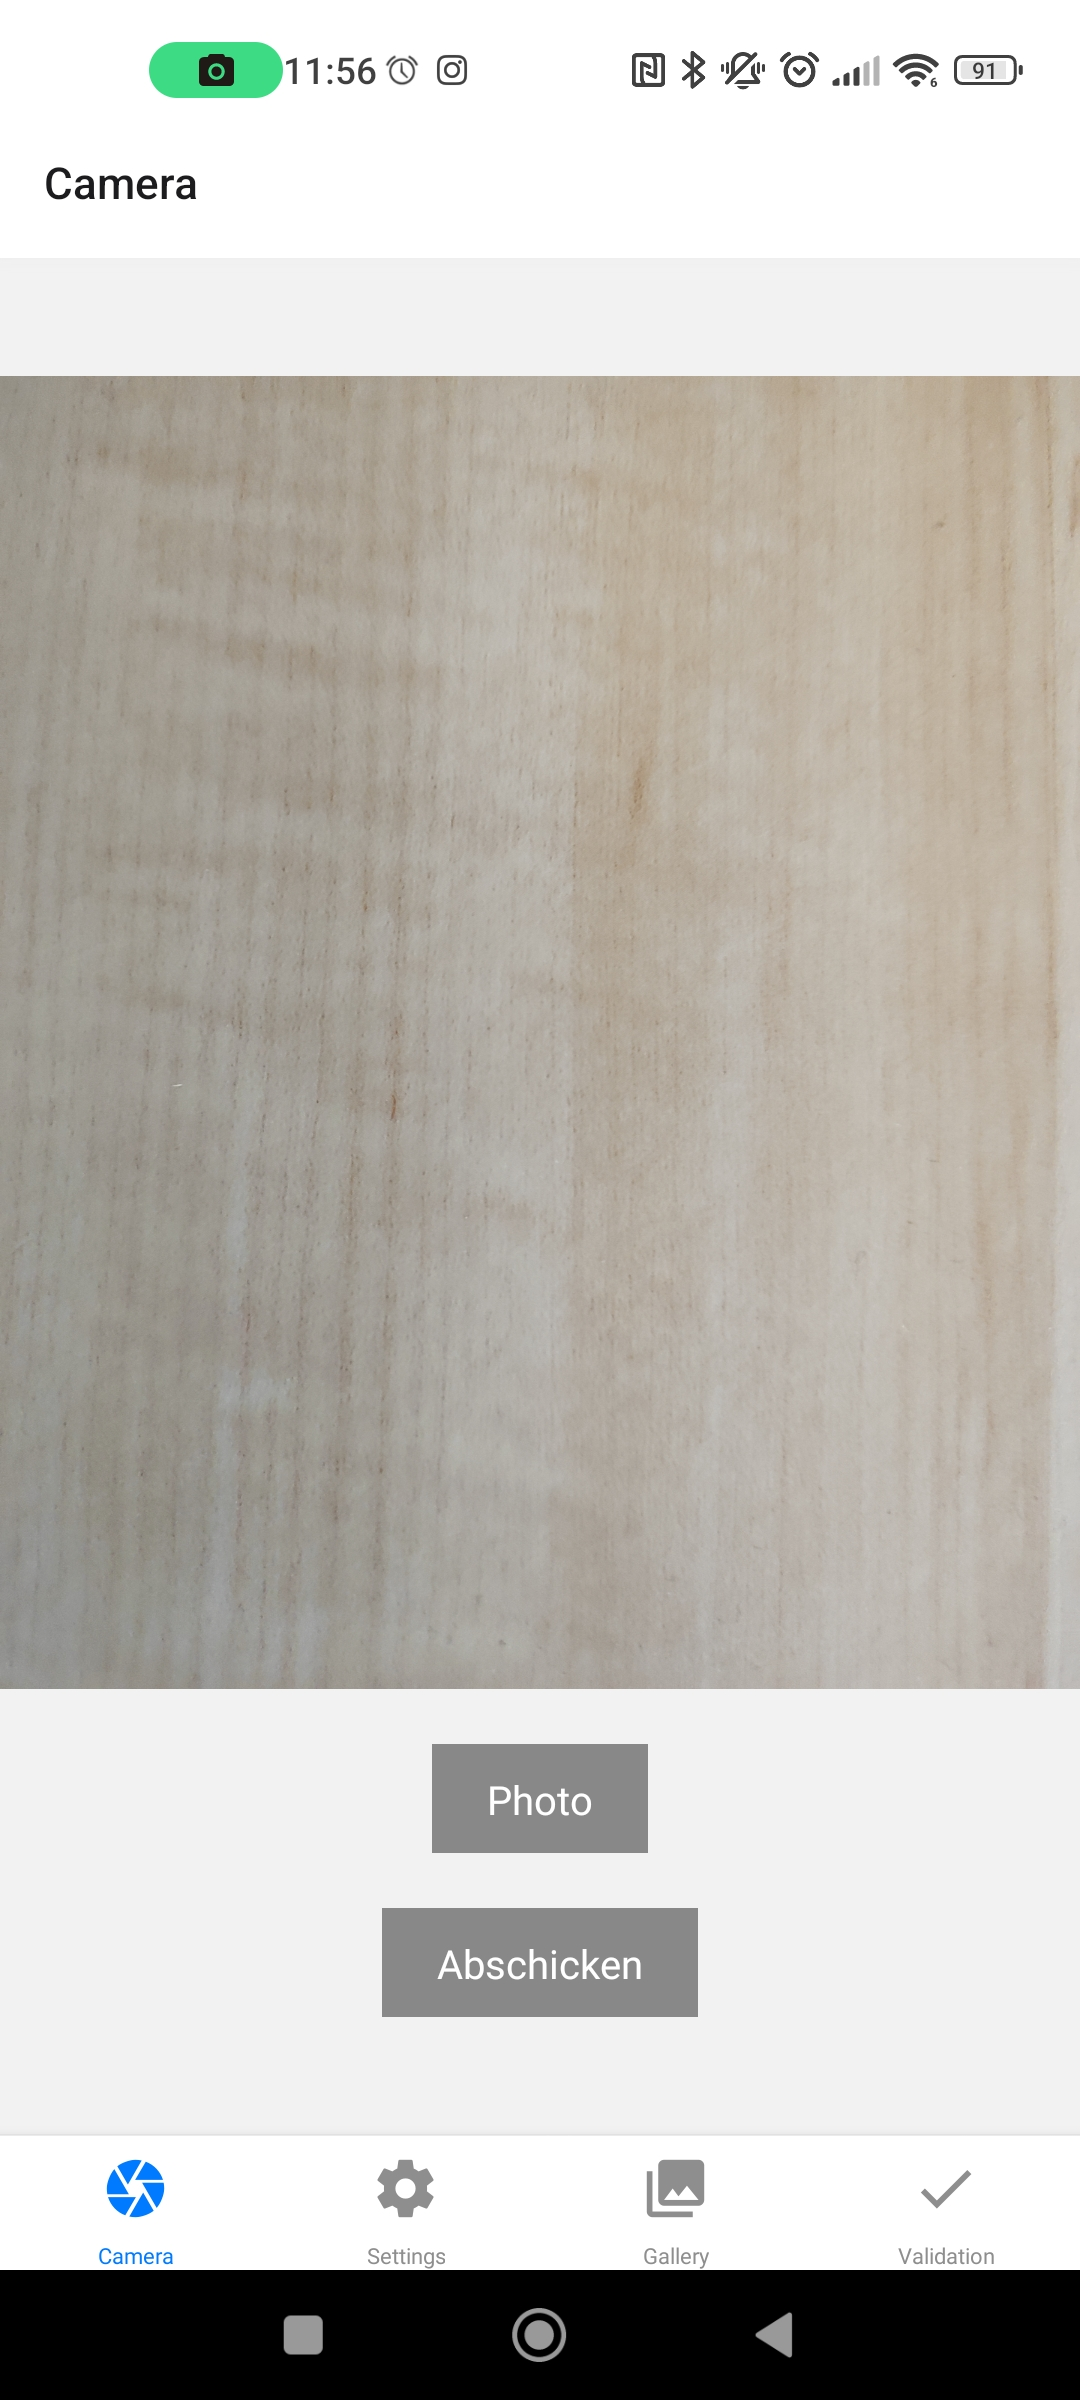
\includegraphics[scale=0.2]{pics/CameraScreen.jpg}
    \caption{Camera Screen}
    \label{fig:impl:camscreen}
\end{figure}

\begin{figure}
    \centering
    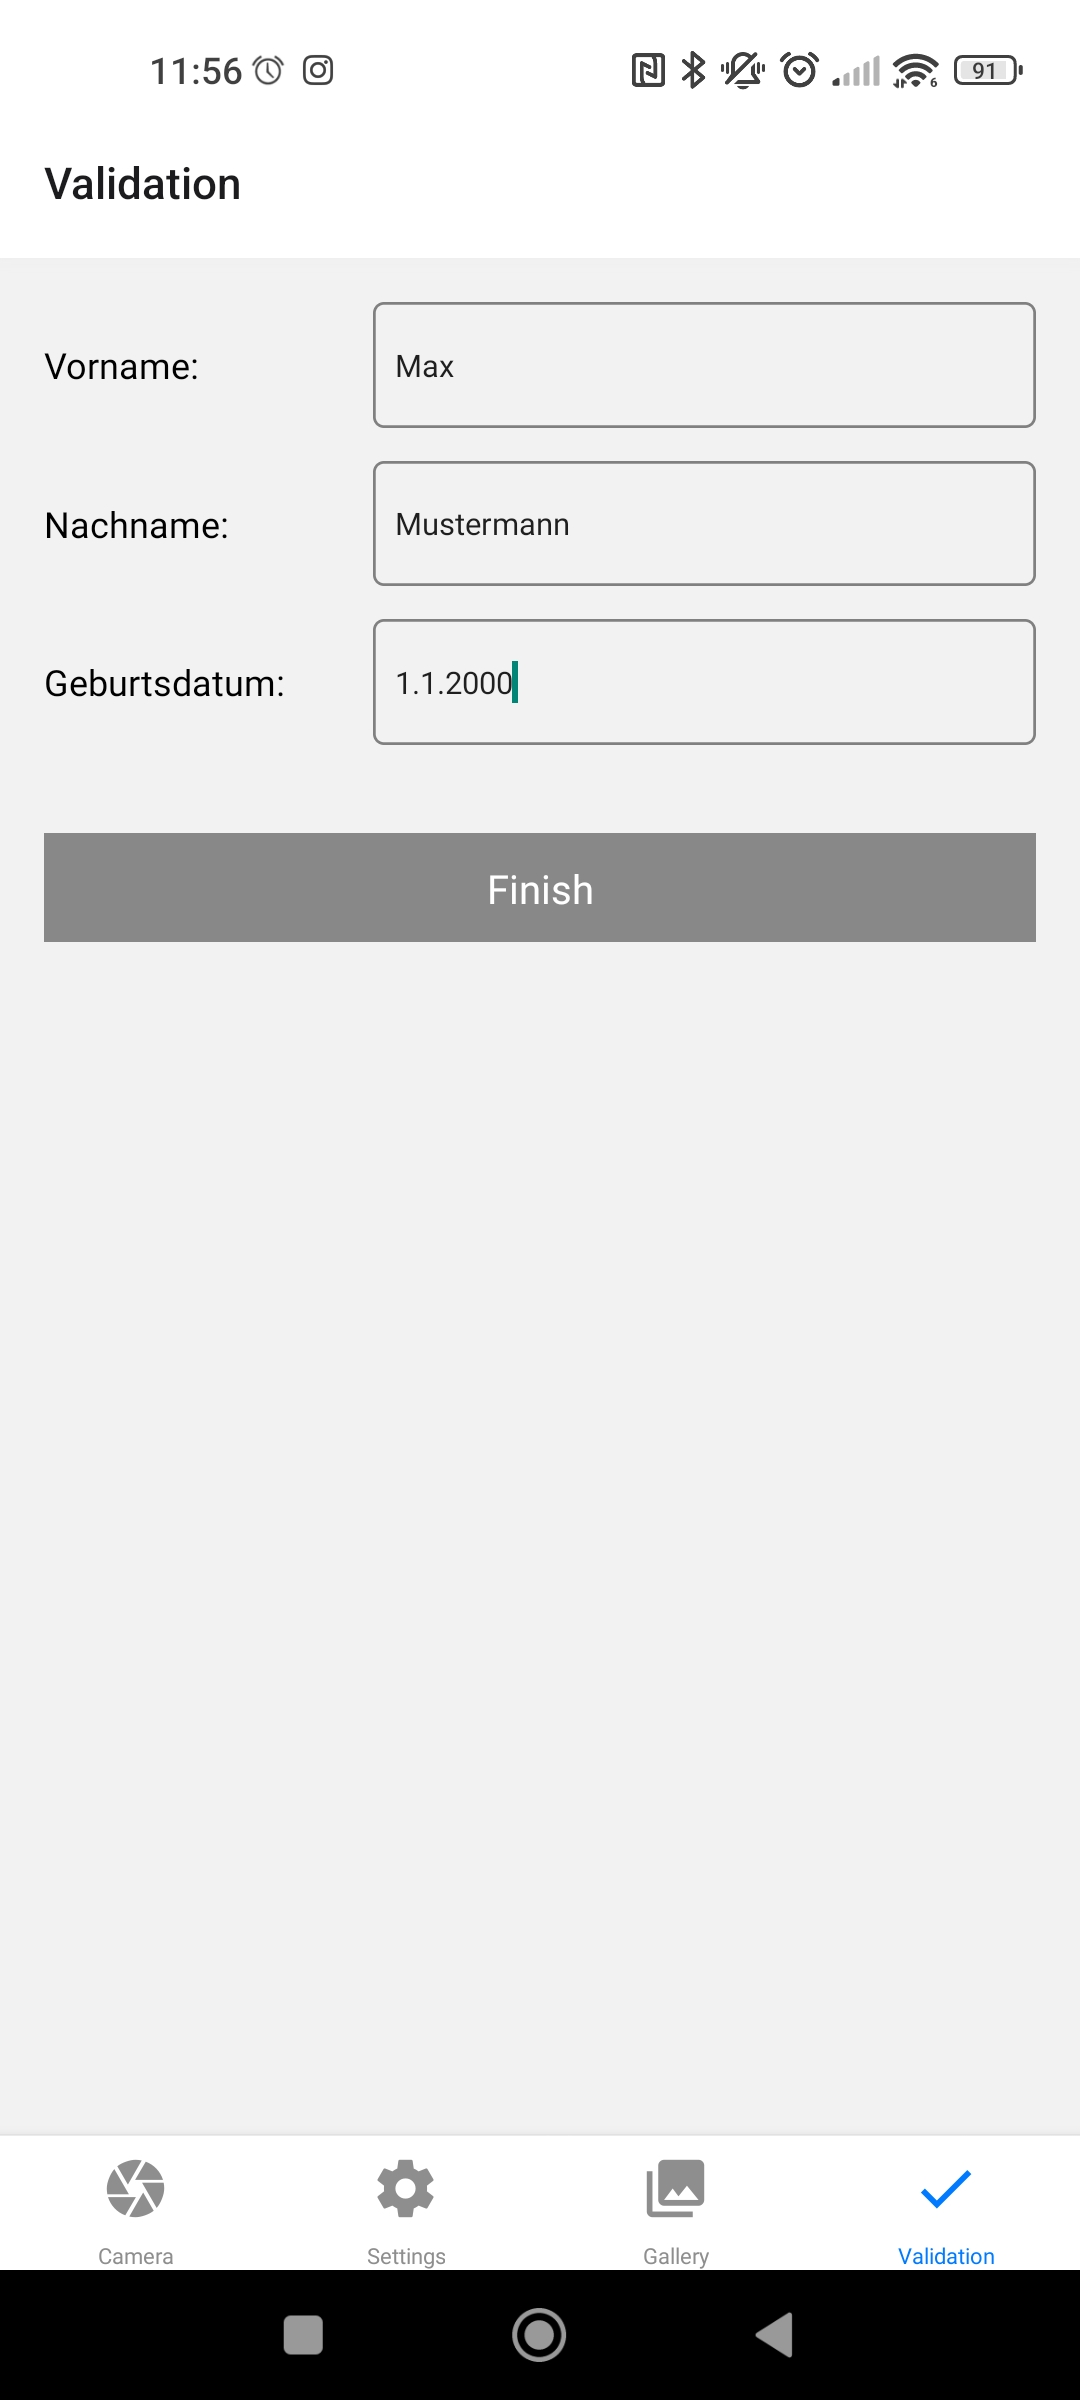
\includegraphics[scale=0.2]{pics/ValidationScreen.jpg}
    \caption{Validation Screen}
    \label{fig:impl:validationscreen}
\end{figure}

\FloatBarrier

\section{Access data entry}


